\section{Detektion}
Zur Überprüfung der Genauigkeit der Kugeldetektion wurden 50 Testbilder von verschiedenen Spielständen aufgenommen
und von Hand die Positionen der Kugeln in Pixelkoordinaten angegeben.
Die Pixelkoordinaten wurden anschliessend in Modellkoordinaten umgewandelt \cite{project2:pixel_to_model_coordinates}.
Diese Referenzdaten können mit dem Resultat des Detektionsalgorithmus verglichen werden,
indem dieser die Kugeln auf denselben Bildern detektiert, auf dieselbe Weise in Modellkoordinaten umwandelt und
die Positionen mit den Referenzdaten verglichen werden.
Die Distanzen zwischen den Kugelpositionen in den Referenzdaten und in der Detektion können
anschliessend statistisch ausgewertet werden.

In den 50 Referenzbildern sind insgesamt 835 Kugelpositionen hinterlegt, in Tabelle \ref{tab:detektion_resultate_distanzen_stats}
sind einige statistische Kennzahlen aus diesem Vergleich aufgeführt. Der Median liegt bei ca. 2.33mm und 50\% der Detektionen
haben einen Positionsfehler zwischen ca. 0mm - 3.7mm. Die maximale Abweichung zwischen Referenzdaten und Detektion liegt bei 8.35mm.

\begin{table}[ht]
    \rowcolors{1}{\seccolor!10}{\seccolor!10} % Rows with 10% of secondary color
    \begin{tabular}{ rrrrrr }
        \rowcolor{\seccolor!50}
        Anzahl Kugeln & Minimum & Unteres Quartil & Median & Oberes Quartil & Maximum\\
        835 & 0.000004mm & 0.000601mm & 2.329217mm & 3.680264mm & 8.3566mm
    \end{tabular}
    \caption{Statistische Zahlen zu den Distanzen zwischen den Kugelpositionen der Referenzdaten und den detektierten Kugelpositionen.}
    \label{tab:detektion_resultate_distanzen_stats}
\end{table}

% Pixel distance: count=624, min=0.000000, lower quartile=1.000000, median=1.414214, upper quartile=2.236068, max=5.099020
% Model distance: count=835, min=0.000004, lower quartile=0.000601, median=2.329217, upper quartile=3.680264, max=8.356600

In Abbildung \ref{fig:detection_results_bad_detections} sind die beiden grössten Detektionsfehler abgebildet.
Dabei handelt es sich um Fälle, wo die detektierte Pixelposition um bis zu 5 Pixel Abweichung gegenüber den Referenzdaten aufweist.
Aus diesen Abweichungen in Pixeln sind Abweichungen bis maximal 8.35mm entstanden.

\begin{figure}[h!]
    \centering
    \begin{subfigure}[t]{0.3\textwidth}
        \centering
        
\includegraphics[width=1.0\linewidth]{../common/04_results/resources/bad_detection_4_8.356600_5.099020.png}
        \caption{Detektionsfehler einer roten Kugel von 5 Pixel und 8.35mm}
        \label{fig:detection_results_bad_detection_1}
    \end{subfigure}
    \begin{subfigure}[t]{0.3\textwidth}
        \centering
        
\includegraphics[width=1.0\linewidth]{../common/04_results/resources/bad_detection_5_7.727108_4.472136.png}
        \caption{Detektionsfehler einer pinken Kugel von 4.47 Pixel und 7.72mm}
        \label{fig:detection_results_bad_detection_2}
    \end{subfigure}
    \caption{
        Die grössten festgestellten Fehler in der Positionsdetektion. Gelb ist die detektierte Kugelposition, türkis die Position aus den Referenzdaten.
        Ein gewisser Fehler in den Referenzdaten ist bei diesen Positionen ist nicht ausgeschlossen.
    }
    \label{fig:detection_results_bad_detections}
\end{figure}

In Tabelle \ref{tab:detektion_resultate_distanzen_stats_pro_kugelfarbe} wurden die Positionsfehler der Detektion
gegenüber den Referenzdaten pro Kugelfarbe ausgewertet.
Es wurden lediglich 32 der 50 Referenzbilder verwendet, da bei den Anderen die korrekten Farben der Kugeln nicht hinterlegt wurden.
Es gibt bei den meisten Kugelfarben keine grossen Unterschiede zu den Zahlen in Tabelle \ref{tab:detektion_resultate_distanzen_stats}.
Lediglich bei den Kugelfarben gelb und grün liegt der Median tiefer als bei allen anderen Kugelfarben.

\begin{table}[ht]
    \rowcolors{1}{\seccolor!10}{\seccolor!10} % Rows with 10% of secondary color
    \begin{tabular}{ lrrrrrrr }
        \rowcolor{\seccolor!50}
        Kugelfarbe & Anzahl Kugeln & Minimum & Unteres Quartil & Median & Oberes Quartil & Maximum\\
        BROWN & 32 & 0.000153mm & 1.682379mm & 2.454655mm & 3.740010mm & 5.395337mm \\
        PINK & 32 & 0.000076mm & 1.678389mm & 2.338619mm & 3.422637mm & 7.727108mm \\
        RED & 224 & 0.000004mm & 1.672397mm & 2.358258mm & 3.659417mm & 8.356600mm \\
        BLACK & 32 & 0.000218mm & 1.685366mm & 2.377796mm & 3.794632mm & 4.688987mm \\
        YELLOW & 32 & 0.000011mm & 1.685552mm & 1.716131mm & 3.393303mm & 5.378226mm \\
        WHITE & 32 & 0.000086mm & 1.677719mm & 2.357014mm & 3.775538mm & 5.394620mm \\
        BLUE & 32 & 0.000071mm & 1.684771mm & 2.351218mm & 3.419713mm & 5.391995mm \\
        GREEN & 32 & 0.000041mm & 0.000356mm & 1.707863mm & 3.703774mm & 7.039578mm
    \end{tabular}
    \caption{Statistische Zahlen zu den Distanzen zwischen den Kugelpositionen der Referenzdaten und den detektierten Kugelpositionen pro Kugelfarbe.}
    \label{tab:detektion_resultate_distanzen_stats_pro_kugelfarbe}
\end{table}

Die verwendete Vergleichsmethode enthält an sich bereits einen Fehlerbereich, welcher der Auflösung des Bildes geschuldet ist.
Eine genaue Beschreibung ist in \cite{project2:fehler_grundwahrheit} enthalten, hier werden die wichtigsten Erkenntnisse
erneut aufgeführt.
Die Ausmasse des Spielbereichs des Billardtisches betragen 1881mm mal 943mm, die Auflösung des Bildes beträgt 1280x720 Pixel.
Der Spielbereich füllt nicht die gesamte Bildauflösung, sondern lediglich 1118x565 Pixel.
Ein einzelnes Pixel des Bildes entspricht damit einer Fläche von 1.681mm mal 1.668mm.
Der Detektionsalgorithmus detektiert die Kugelpositionen subpixelgenau.
Die maximale Abweichung unter der Annahme, dass das korrekte Pixel in den Referenzdaten angegeben wurde, beträgt 1.18406mm.

Die Annahme, dass in den Referenzdaten das korrekte Pixel angegeben wurde, ist selbstverständlich höchst unwahrscheinlich.
In Abbildung \ref{fig:detektion_resultate_min_max_fehler_referenzdaten} sind verschiedene Fälle aufgeführt,
um eine Aussage darüber zu machen, wie sich ein Fehler in den Referenzdaten auf deren Genauigkeit auswirkt.

\begin{figure}[h!]
    \begin{center}
        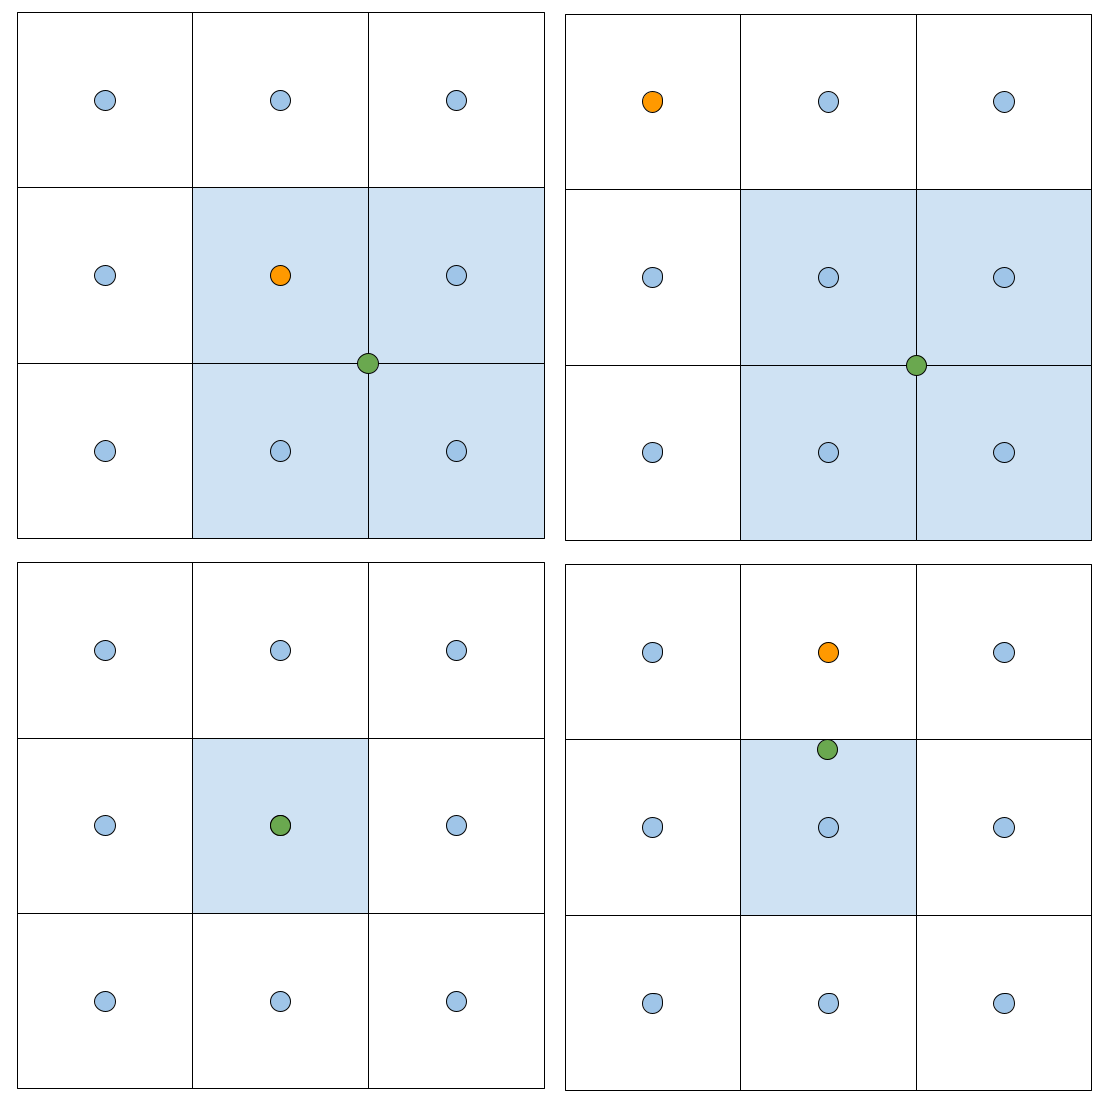
\includegraphics[width=0.5\linewidth]{../common/04_results/resources/detektion_min_und_max_fehler.png}
    \end{center}
    \caption{
        Extremsituationen zum Vergleich der Referenzposition und der wahren Position des Kugelmittelpunktes.
        Abgebildet ist ein Bildausschnitt mit 9 Pixeln. Die blauen Punkte sind die Pixelzentren, grün ist die wahre Position (subpixelgenau), orange ist die Referenzposition aus den Referenzdaten.
        Die Pixel rund um die wahre Position sind blau hinterlegt.
        Oben-Links: Der maximale Fehler ist eine halbe Pixeldiagonale, wenn die wahre Position zwischen vier Pixeln liegt und die Referenzposition einem der Pixel rund um die tatsächliche Position entspricht.
        Unten-Links: Der minimale Fehler ist $0$, wenn die wahre Position genau dem Pixelzentrum entspricht und dieses Pixel in den Referenzdaten ausgewählt wurde.
        Oben-Rechts: Der maximale Fehler ist 1.5 Pixeldiagonalen, wenn die wahre Position zwischen vier Pixeln liegt und die Referenzposition um ein Pixel daneben ist.
        Unten-Rechts: Der minimale Fehler ist eine halbe Pixelbreite/-höhe wenn die wahre Position innerhalb des zentralen Pixels liegt und die Referenzposition um ein Pixel falsch daneben ist.
    }
    \label{fig:detektion_resultate_min_max_fehler_referenzdaten}
\end{figure}

In Abschnitt \ref{kap:tracking} wurde beschrieben, dass in der Live-Detektion eine Stabilisierung der detektierten Positionen
über die Zeit durchgeführt wird.
In diesem Kapitel wurden nur Bilder für den Vergleich zwischen Detektion und Realität verwendet, wodurch es sich um Momentaufnahmen handelt.
Es kann sein, dass die Stabilisierung in gewissen Fällen die detektierten Positionen verbessert,
weil Positionsfehler in einzelnen Bilder geglättet werden.

Die implementierte Live-Detektion gilt es nachfolgend ebenfalls zu überprüfen.

Ein Problem der Live-Detektion ist, dass wenn ein Spieler mit der Hand in das Bild greift, um u.a. einen Stoss
durchzuführen, dann werden bei der Hand ebenfalls Kugeln detektiert, siehe Abbildung \ref{fig:detection_hand_problem}.
Dies ist darauf zurückzuführen, dass die Detektion eine Segmentierung des HSV-Farbraumes durchführt\cite{project2:snooker_detection}
und anschliessend darauf den Circle Hough transform\cite{wiki:circle_hough} ausführt.
Dadurch werden Kleider oder Haut ebenfalls als Bereiche erkannt, wo eine Kugel sein könnte. Der Circle Hough transform
findet anschliessend aufgrund von Kanten in diesen Bereichen Kreise, welche dann als detektierte Kugeln übernommen werden.

\begin{figure}[h!]
    \begin{center}
        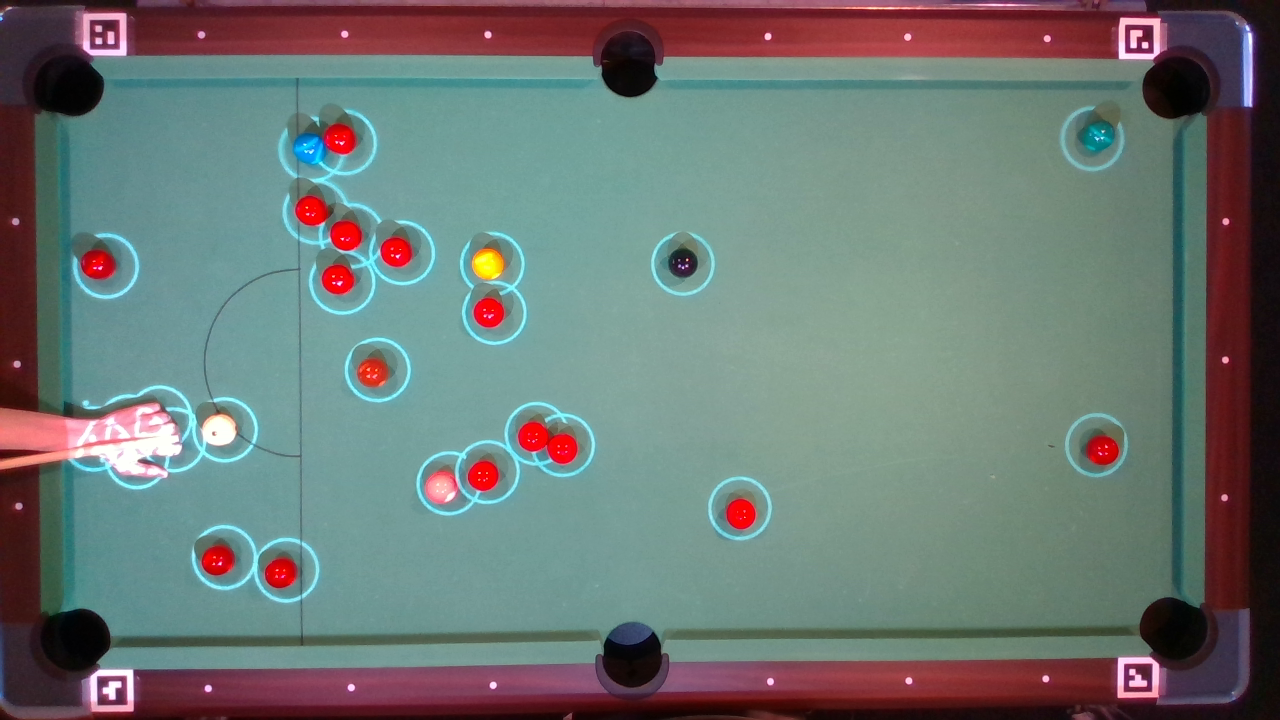
\includegraphics[width=0.8\linewidth]{../common/04_results/resources/detektierte_kugeln_auf_der_hand.png}
    \end{center}
    \caption{Fälschlicherweise detektierte Kugeln auf der Hand}
    \label{fig:detection_hand_problem}
\end{figure}

Sofern die Arme und Hände des Spielers segmentiert werden könnten, wäre es möglich diese Fehler in der Detektion zu verhindern.
Dazu würden die segmentierten Regionen, wo eine Hand oder ein Arm abgebildet ist, in der Detektion ignoriert.
Diese Segmentation ist allerdings schwierig durchzuführen, da diese stark von Hautfarbe und Bekleidung abhängt.
Es wäre hier denkbar, ein vortrainiertes neuronales Netzwerk zu verwenden, welches eine Handsegmentation oder -detektion machen kann.

Das in Abschnitt \ref{kap:tracking} beschriebene Tracking zur Stabilisierung der Kugelpositionen hat zu einer deutlichen
visuellen Verbesserung geführt.
Sofern der Spielstand ruhig ist, also keine Kugeln in Bewegung sind, bewegen sich die
projizierten Kreise rund um die detektierte Position kaum noch.
Ohne Tracking ist das Rauschen in der detektierten Position anhand der bewegenden Kreise sichtbar.

Diese visuelle Verbesserung kann auch statistisch quantifiziert werden, indem die Detektion auf einem Video eines
ruhigen Spielstandes durchgeführt wird. Die Detektion kann auf jedem einzelnen Frame des Videos durchgeführt werden, und
die detektierte Position mit derjenigen im vorherigen Frame verglichen werden.
Die Distanz zwischen der detektierten Position in Frame $F_{t-1}$ und derjenigen in Frame $F_{t}$ bildet anschliessend
eine Messung, die gesammelt wird.

Auf den gesammelten Distanzen können anschliessend statistische Kennzahlen berechnet werden.
Diese Messungen wurden mit und ohne Stabilisierung der Kugelpositionen durchgeführt, die Resultate sind in Tabelle \ref{tab:detektion_resultate_tracking_stats} aufgeführt.
Die Messungen basieren auf einem Videoausschnitt von 178 Frames eines Videos mit einem Spielstand wo 21 Kugeln stillstehen.
Die Messung wurde erst nach 30 Frames gestartet, damit die Messung mit eingeschalteter Stabilisierung bereits einige
Daten sammeln konnte.
Während dieser Aufwärmphase wäre die Detektion mit eingeschalteter Stabilisierung anfällig auf Rauschen in der Detektion,
wie es die Detektion ohne Stabilisierung ist.
Durch diesen Vorlauf von 30 Frames beträgt der gemessene Videoausschnitt 148 Frames.
Dies resultiert in $148 \cdot 21 = 3108$ Messwerten.
Aus Tabelle \ref{tab:detektion_resultate_tracking_stats} wird klar, dass die Stabilisierung die Bewegung der
detektierten Kugelpositionen deutlich verringern konnte.

\begin{table}[ht]
    \rowcolors{1}{\seccolor!10}{\seccolor!10} % Rows with 10% of secondary color
    \begin{tabular}{ lrr }
        \rowcolor{\seccolor!50}
        Bezeichnung & Stabilisierung ausgeschaltet & Stabilisierung eingeschaltet\\
        Anzahl Messwerte & 3108 & 3108\\
        Minimum & 0mm & 0mm\\
        Unteres Quartil $Q_{0.25}$ & 1.638916mm & 0.081972mm\\
        Median $Q_{0.5}$ & 2.359856mm & 0.129632mm\\
        Oberes Quartil $Q_{0.75}$ & 3.714067mm & 0.222898mm\\
        Quartilabstand $Q_{0.75} - Q_{0.25}$ & 2.075151mm & 0.140926mm\\
        Maximum & 13.590104mm & 4.043161mm\\
        Summe aller Messungen & 7654.91mm & 588.849mm
    \end{tabular}
    \caption{
        Statistische Zahlen zu der Verteilung der Veränderung der detektierten Kugelpositionen über eine Dauer von
        148 Video-Frames mit und ohne Stabilisierung.
        Bei einem Messwert handelt es sich um die Distanz zwischen der detektierten Kugelposition in Frame $F_{t-1}$
        und Frame $F_{t}$ für eine Kugel.
    }
    \label{tab:detektion_resultate_tracking_stats}
\end{table}
% ohne stabilisierung: Total delta movement summary: count=3108 min=0.000000, lower quartile=1.638916, median=2.359856, upper quartile=3.714067, max=13.590104
% mit  stabilisierung: Total delta movement summary: count=3108 min=0.000000, lower quartile=0.081972, median=0.129632, upper quartile=0.222898, max=4.043161
% ohne stabilisierung: Total delta movement: 7654.91mm, 148 frames, lost: 0
% mit  stabilisierung: Total delta movement: 588.849mm, 148 frames, lost: 0

In Abbildung \ref{fig:detektion_resultate_tracking_boxplot} sind die Daten aus Tabelle \ref{tab:detektion_resultate_tracking_stats}
in zwei Box-Plot-Diagrammen visualisiert.

\begin{figure}[h!]
    \begin{center}
        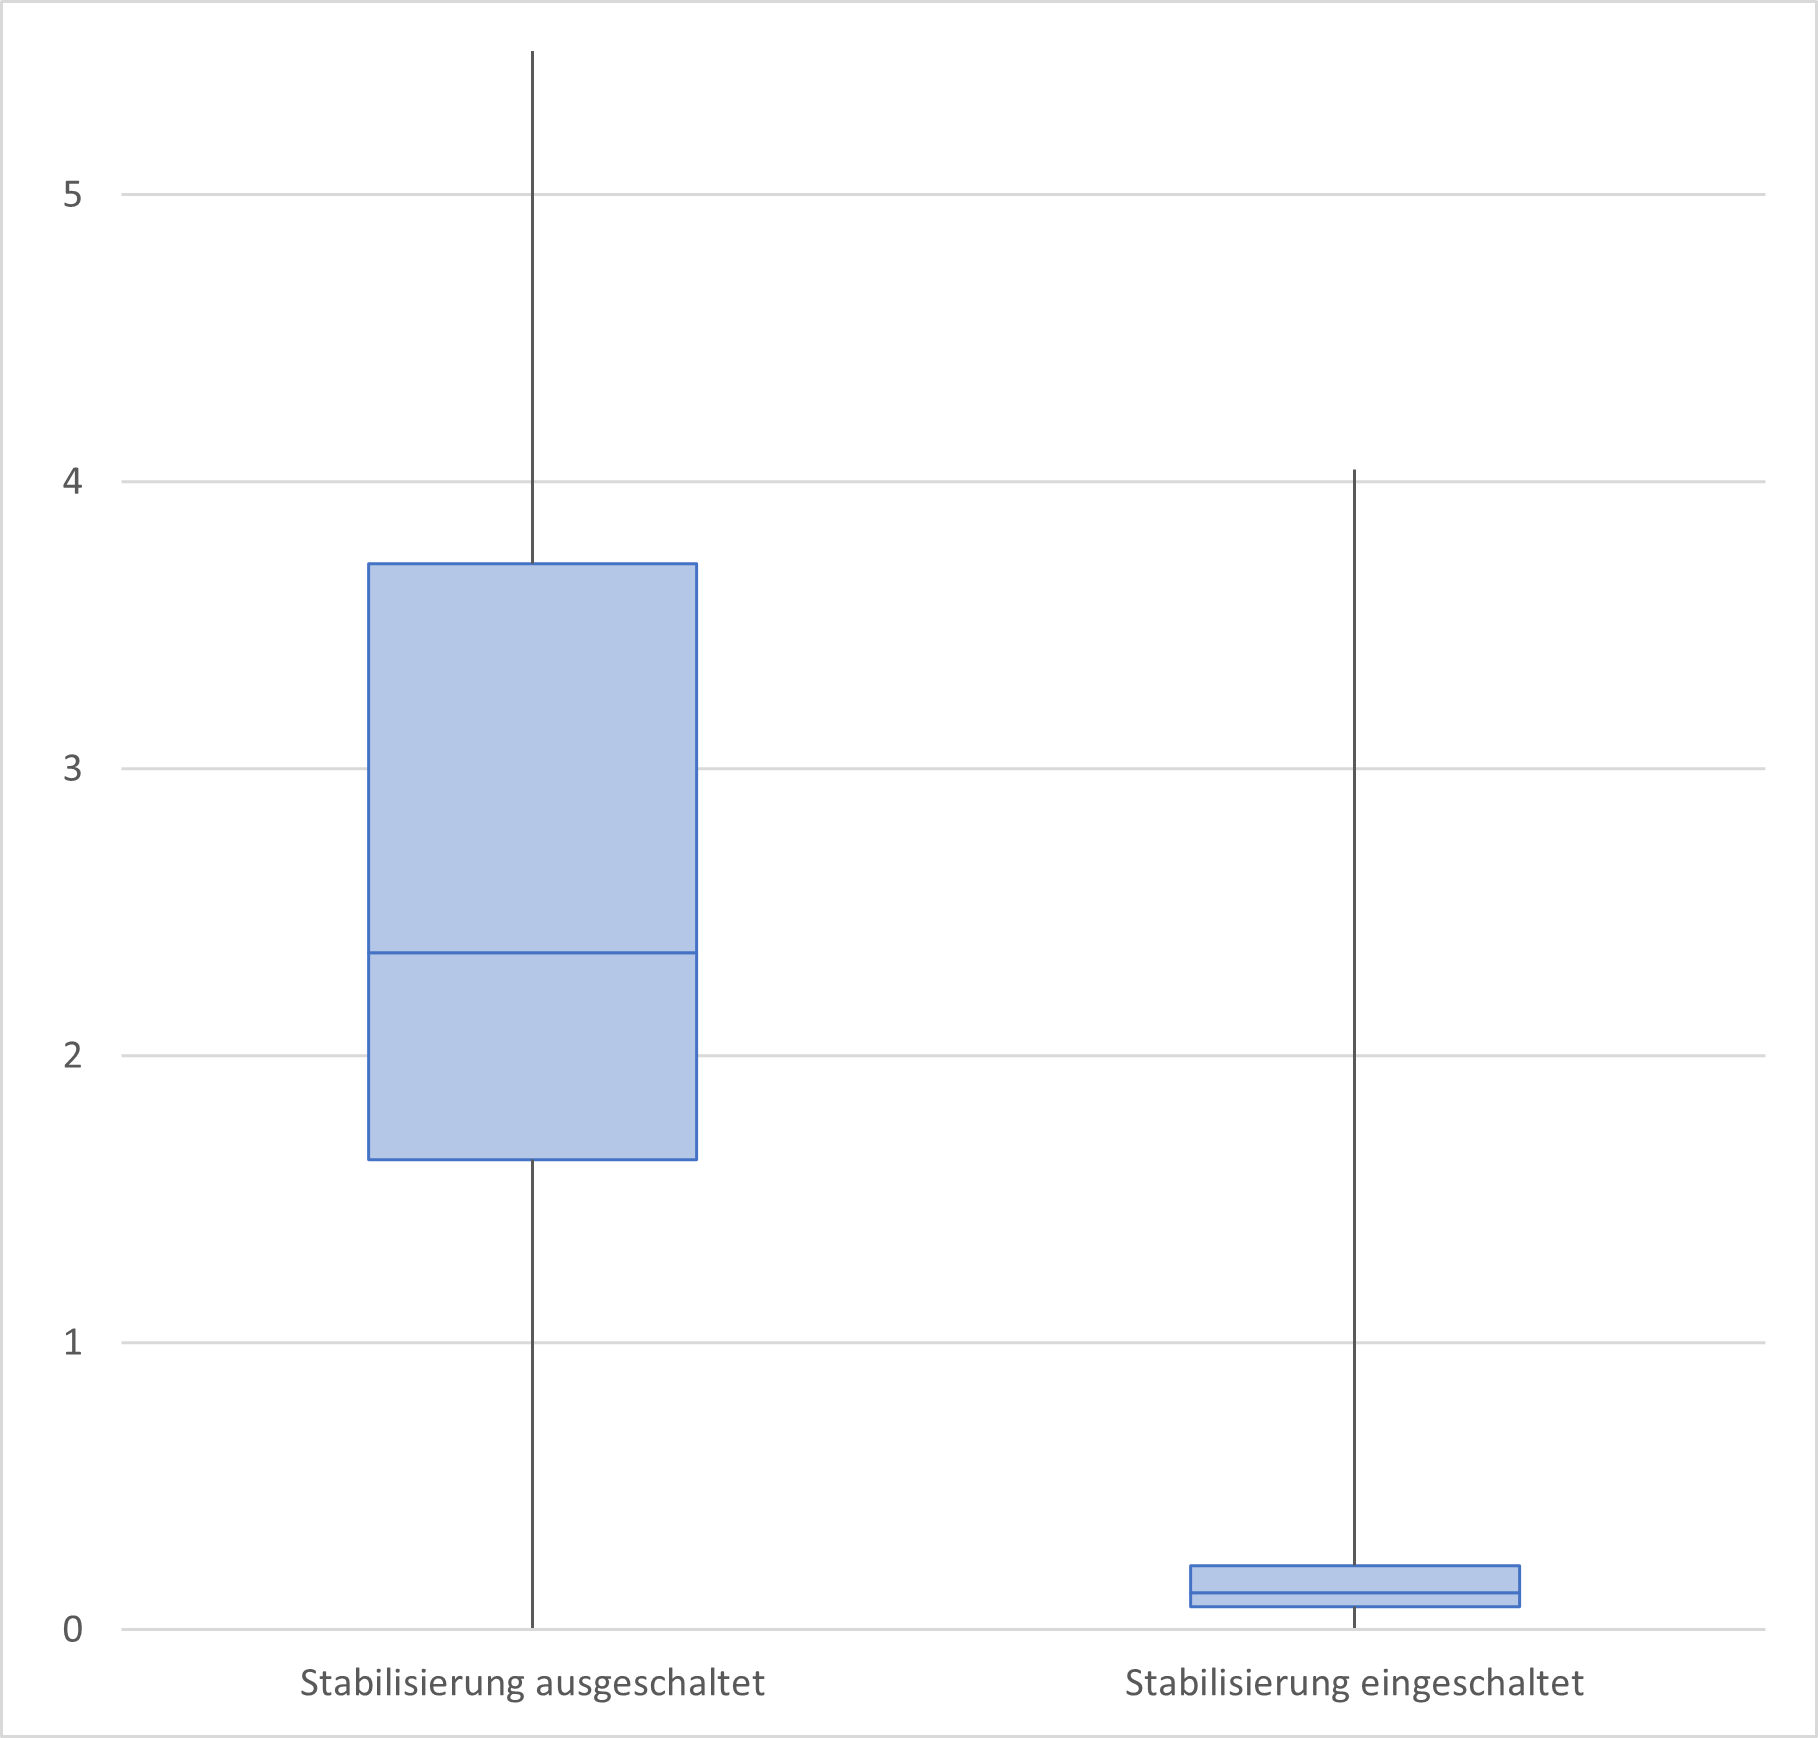
\includegraphics[width=0.5\linewidth]{../common/04_results/resources/stabilisierung_boxplot.png}
    \end{center}
    \caption{
        Box-Plot-Diagramme zu der Bewegung der Kugelpositionen mit und ohne Stabilisierung
        gemäss Tabelle \ref{tab:detektion_resultate_tracking_stats}.
        Der Wertebereich der Y-Achse wurde auf 5 beschränkt, damit das rechte Diagramm ersichtlich ist.
        Die Antenne des linken Diagrammes geht bis zum Maximum von 13.59mm.
    }
    \label{fig:detektion_resultate_tracking_boxplot}
\end{figure}
